\chapter{Theoretical Background}
This chapter introduces the fundamental concepts used throughout this thesis. It explains key definitions and presents an overview of BERT, focusing on the features necessary for building the detection system.

% --------------------------------------------------------------------------------

\section{Definitions}
\subsection{Natural Language Processing and Machine Translation}
    \textbf{NLP} enables machine systems to process human language. The goal is to mimic and understand it as fluently as possible \parencite{smacchiaDoesAIReflect2024,ullmannGenderBiasMachine2022}. Common applications are chatbots, translation tools, speech recognition, and image captioning. \textbf{MT} is a direct application of NLP. It performs automatic translation of text from one language to another \parencite{linMachineTranslationAcademic2009}. Over time, MT systems have developed from rule-based approaches, which depend on hand-crafted grammar rules or aligned sentence data, into more adaptable neural models \parencite{chakravarthiSurveyOrthographicInformation2021}.

    Most modern systems, such as Google Translate and DeepL, rely on neural machine translation (NMT) \parencite{wuGooglesNeuralMachine2016,deeplHowDoesDeepL2021}. These models are trained on large collections of translated texts. They learn to represent the meaning of entire sentences as mathematical structures, enabling more fluent and accurate translations. Unlike earlier approaches, NMT systems take the full sentence context into account, which helps reduce errors and improves the handling of ambiguous or idiomatic language \parencite{wuGooglesNeuralMachine2016}. Throughout this work, all MT systems referenced or applied are neural models.

\subsection{Bias and its Manifestations}
\label{subsection:manifestations_of_gb}
    Bias refers to a tendency to favour or disadvantage certain individuals or groups based on preconceived ideas. It often comes from stereotypes, which are fixed and oversimplified ideas about a group. In short, stereotypes shape assumptions, while bias influences actual behavior and treatment.

    Bias takes many forms and can be based on characteristics such as age, disability, gender, ethnicity, religion, or sexual orientation \parencite{ullmannGenderBiasMachine2022}. These biases frequently originate from longstanding cultural and historical beliefs about the expected behavior of different groups. This thesis focuses specifically on gender bias, which is particularly prominent in MT due to the influence of gendered language. Elements such as gendered terms, occupational roles, and grammatical patterns can affect translations and often perpetuate stereotypes because language is closely tied to our thoughts and beliefs. Drawing on key studies that examine gender bias in EN-DE MT \parencite{ullmannGenderBiasMachine2022,rescignoGenderBiasMachine2023,lardelliBuildingBridgesDataset2024,kapplAreAllSpanish2025}, such bias typically manifests in the following forms:

    \subsubsection{Defaulting to Masculine Forms}
        In both singular and plural contexts, the \textit{generic masculine} uses the masculine grammatical gender as the default.
        For example, the sentence "Die Studenten sind im Hörsaal" (The students are in the lecture hall) uses the masculine plural form to refer to a group of students regardless of their gender. It is commonly used in spoken German and other gendered languages \parencite{lardelliBuildingBridgesDataset2024,schmitzGermanAllProfessors2022}, although research has consistently shown that the generic masculine creates a male bias in mental representations, leading readers or listeners to think more of male than female examples \parencite{sczesnyCanGenderFairLanguage2016}. 

    \subsubsection{Reinforcement of Stereotypes}
        The gendered language patterns discussed earlier reflect broader social beliefs about men’s and women’s roles in work and family life. Although many of these roles no longer reflect reality, they continue to shape judgments about people’s abilities and personalities. This often leads to correspondence bias, where traits are inferred based on behavior or circumstances \parencite{godsilEffectsGenderRoles2016}. Such stereotypes are reinforced by media, including television and advertising, and influence how language is used and understood. One common result of this is stereotypical job associations. People often link roles like doctors or pilots with he/him pronouns, and roles like nurses or flight attendants with she/her pronouns \parencite{shresthaExploringGenderBiases2022}. \textcite{pratesAssessingGenderBias2019} also found clear patterns in how gender is associated with certain traits. Adjectives like "shy," "happy," "kind," and "ashamed" are often linked to women, while words like "arrogant," "cruel," and "guilty" are more often linked to men. 

  
 \subsection{Gender Bias} \label{subsection:definition_gb}
    A clear definition of gender bias in MT does not exist, nor is there a standard method to identify indicative features in text \parencite{barclayInvestigatingMarkersDrivers2024a}. This leads this study to use a simple rule-based definition to determine when a translation of a sentence is gender biased.

        \begin{itemize}
        \item A gender-ambiguous subject in the source text is translated with a gendered term, often by defaulting to the generic masculine (e.g., doctor → Arzt) or reflecting stereotypical gender roles (e.g., nurse → Krankenschwester).
        \item A gendered subject in the source text is assigned an incorrect gender in the translation, leading to semantic inconsistency (e.g., my mother is an engineer → meine Mutter ist ein Ingenieur).
        \end{itemize}

    This does not mean that all other cases are truly "unbiased". I will refer to anything that does not fall under these two cases as "neutral". This includes, but is not limited to:

        \begin{itemize}
        \item Sentences with no gendered terms, like "The weather is nice".
        \item Accurate translations of gendered input, like "The woman is a coder" → "Die Frau ist eine Programmiererin".
        \item The use of gender-fair alternatives (see \autoref{subsection:german_gfl}).
        \end{itemize}

    \begin{table}[htb]
    \centering
    \begin{tabularx}{\linewidth}{X | X}
        \toprule
        \textbf{Biased Translation} & \textbf{Neutral/Fair Translation} \\
        \midrule
        Gender-ambiguous source is translated with a gendered term. & 
        Gender ambiguity is preserved in the translation. \\
        \addlinespace[0.5em]
        Gendered subject is assigned an incorrect gender. & 
        Gender in the translation matches the gendered subject. \\
        \addlinespace[0.5em]
        \multicolumn{1}{c|}{—} & 
        Use of gender-fair language alternatives (see \autoref{subsection:german_gfl}). \\
        \bottomrule
    \end{tabularx}
    \caption[Summary of gender bias scenarios in translation]{Summary of gender bias scenarios in translation (original compilation)}
    \label{tab:overview_bias_neutral}
    \end{table}

    \subsection{Binary Classification in NLP}
    Binary classification means sorting items into two clear groups. It is the most common task in ML and is frequently found in every day life, such as automatically flitering e-mails as "spam" or "not spam" \parencite{quemyBinaryClassificationUnstructured2019} or deciding whether a transaction is "fraudulent" or "legitimate". For instance, a spam filter uses previously labeled e-mails to learn relevant patterns, such as specific keywords or sender information, and builds a model that applies these patterns to classify new messages accurately. This thesis tries to label a translation as either "biased" or "neutral". While it is possible to extend the classification beyond two categories to distinguish types of bias or include "gender-fair" labels, doing so would require significantly more data and training. Given the practical aim of this work, the simpler binary approach is more suitable.

    % --------------------------------------------------------------------------------

\section{BERT}
    BERT, which stands for Bidirectional Encoder Representations from Transformers, is a language model that was introduced by Google in 2018 \parencite{devlinBERTPretrainingDeep2019}. After pre-training, BERT can be adapted to many NLP tasks by adding a simple output layer and then fine-tuning the model on task-specific data. The output layer is a small component that produces the final prediction, such as assigning a label to a piece of text. This approach avoids the need for major changes to the original architecture. Its strong ability to understand language makes it well suited for this binary classification tasks. There are multiple variants of the original BERT model. It was originally released in two sizes: \texttt{BERT-Base} and \texttt{BERT-Large}, which differ in the number of layers, attention heads, and overall model capacity \parencite{devlinBERTPretrainingDeep2019}. Since then, many other versions have been developed. Most of them modify either BERT’s pre-training objectives or the underlying Transformer architecture \parencite{libovickyHowLanguageNeutralMultilingual2019}.

\subsection{Transformer Architecture} \label{subsection:transformer_arch}
    The Transformer processes input sequences by transforming them into output sequences using a self-attention mechanism \parencite{phuongFormalAlgorithmsTransformers2022}. This mechanism lets the model weigh the importance of all input elements at the same time \parencite{xiaoIntroductionTransformersNLP2023}, so it can consider every word in a sentence and determine which ones are most relevant to each word. Unlike traditional methods such as Recurrent Neural Networks (RNNs) that process input step by step, self-attention captures global dependencies and contextual relationships more accurately, producing "context-aware" representations.

    The transformer architecture consists of two main components: the encoder and the decoder. The encoder’s job is to read the input sentence and turn it into a series of vectors the model can understand. Each vector is a list of numbers representing the meaning and structure of each word \parencite{xiaoIntroductionTransformersNLP2023}. The encoder works as follows (see \autoref{fig:transformer_architecture}):

    \begin{enumerate}
        \item It receives input embeddings, which represent the words, and positional encodings, which tell the model the order of the words.
        
        \item The data then passes through several identical layers. Each layer has two main components. Each of these is followed by an \textbf{Add \& Layer Norm} step, which helps stabilize and preserve useful information:
        \begin{enumerate}[label=\alph*.]
            \item \textbf{Multi-head self-attention} runs several attention processes in parallel. Each attention head focuses on different details to help the model understand the sentence better.
            \item A \textbf{Feed-forward network} processes each word vector separately, refining the information like a small filter.
    \end{enumerate}
    
    \item Each layer builds on the output of the previous one, helping the model form more complex and abstract ideas about the input sentence.
    
    \item Finally, the encoder outputs a sequence of \textit{hidden states}. These are continuous vector representations for each input token. They encode contextual information from the entire sentence. For example, in the sentence "The cat sat on the mat," the vector for "cat" reflects its relationship to words like "sat" and "mat."
\end{enumerate}

\begin{figure}[ht]
    \centering
	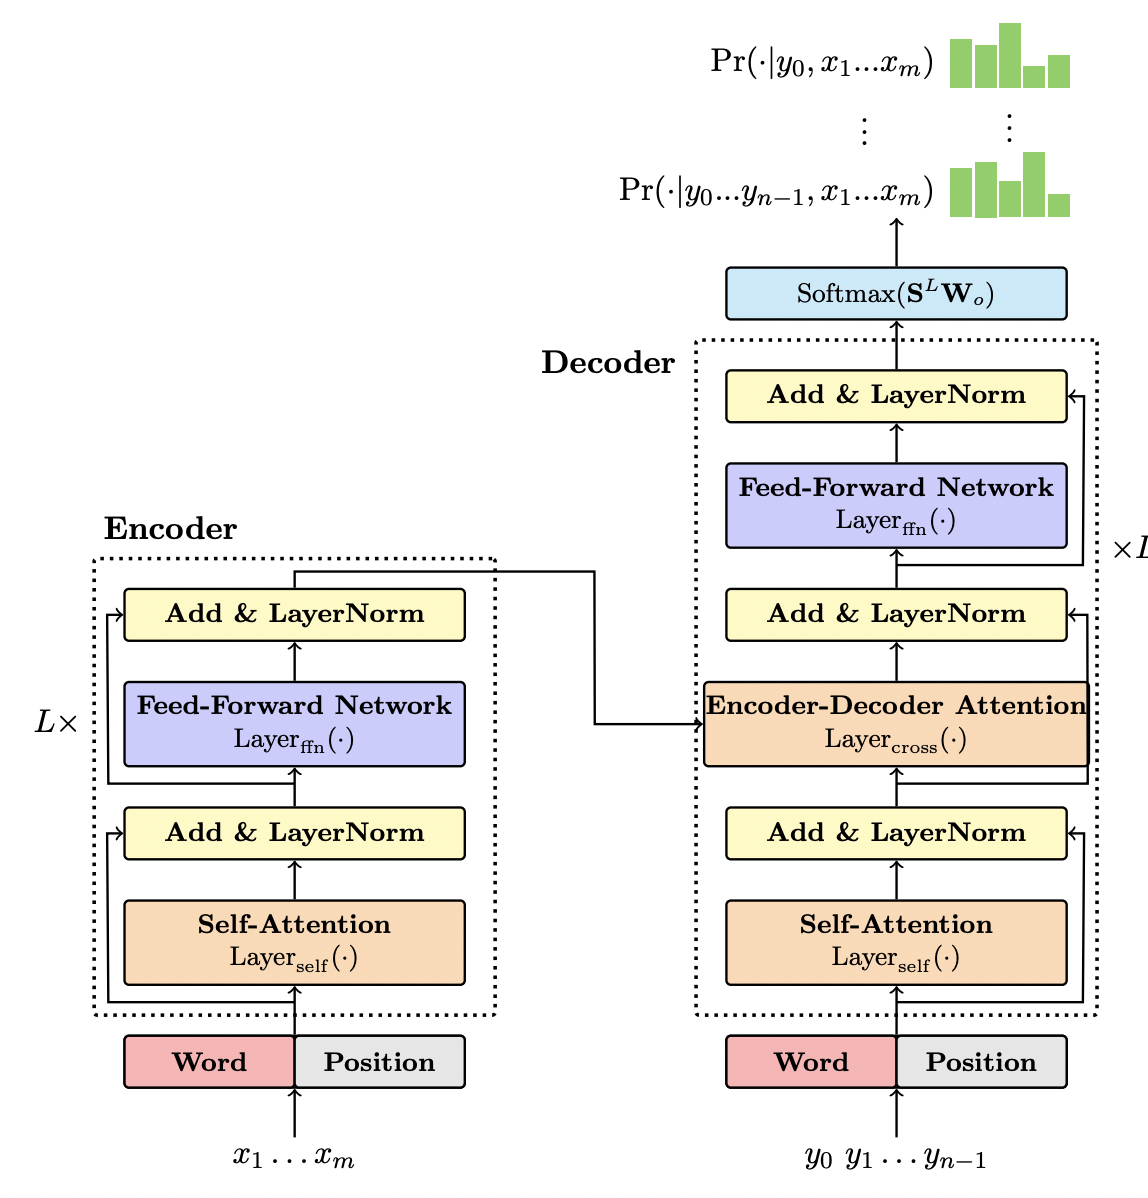
\includegraphics[width=\textwidth,height=0.45\textheight,keepaspectratio]{transformer_architecture.png}	
        \caption[Transformer encoder-decoder architecture overview]{Transformer encoder-decoder architecture. The encoder (left) processes input tokens \(x_1,\dots,x_m\) through: (1) a self-attention layer for contextual relationships, (2) a feed-forward network for feature transformation, and (3) residual connections with layer normalization. The decoder (right) generates outputs by attending to both the encoder's representations and its previous outputs ($y_0$ to $y_{n-1}$), producing the next-token probability distribution. Figure and description adapted from \textcite{xiaoIntroductionTransformersNLP2023}, p. 6}
    \label{fig:transformer_architecture}
\end{figure}

The decoder generates the output sentence one word at a time by using the information from the encoder \parencite{xiaoIntroductionTransformersNLP2023}. However, since BERT uses only an encoder-only architecture (see \autoref{fig:bert_arch}), the decoder is not relevant for this work and is therefore excluded from the discussion.

\subsection{Multilingual BERT}
    In this thesis, the model used is multilingual BERT \textbf{\href{https://huggingface.co/google-bert/bert-base-multilingual-cased}{(\texttt{mBERT})}} \parencite{devlinBERTPretrainingDeep2019}. \texttt{mBERT} has the same architecture as \texttt{BERT-Base} but was pretrained on Wikipedia data from 104 languages, including English and German. The model does not receive any explicit signal about which language it is processing. It is also not trained to align translations across languages. Instead, its multilingual ability emerges from shared patterns it learns across the multilingual corpus \parencite{piresHowMultilingualMultilingual2019}. Despite the lack of cross-lingual supervision, the model develops internal representations that support tasks in multiple languages. Monolingual models like \href{https://huggingface.co/google-bert/bert-base-german-cased}{\texttt{German BERT}} do not support English input. Larger multilingual models, such as \href{https://huggingface.co/docs/transformers/en/model_doc/xlm-roberta}{\texttt{XLM-RoBERTa}}, require more computational resources and training time, which was not feasible here. \texttt{mBERT} offers a good balance between language coverage, model size, and training efficiency, making it a practical choice detecting gender bias in EN-DE translations.

\begin{figure}
    \centering
	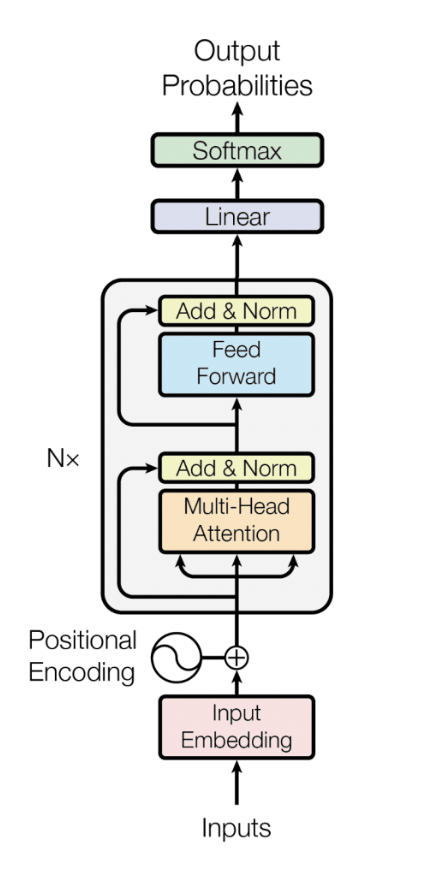
\includegraphics[width=\textwidth,height=0.45\textheight,keepaspectratio]{BERT_architecture.png}	
    \caption[BERT's encoder-only architecture]{BERT's encoder-only architecture Figure by \textcite{smithCompleteGuideBERT2024}}
    \label{fig:bert_arch}
\end{figure}

\subsection{Tokenization}
\texttt{mBERT} processes input by splitting words or subword units into \textit{tokens} (tokenization)\footnote{This tokenization process applies to both BERT and mBERT.}. It uses the WordPiece algorithm with a shared vocabulary of 110,000 tokens \parencite{devlinMultilingualBERTGitHub2018}. To balance the training data, languages with large Wikipedia corpora are downsampled, while those with fewer resources are oversampled. Pre-processing is the same for all supported languages: (1) converting text to lowercase and removing accents, (2) splitting punctuation, and (3) tokenizing based on whitespace. Removing accents helps reduce the vocabulary size, even though it can introduce ambiguity in languages where accents carry meaning. This trade-off is accepted because \texttt{mBERT's} contextual embeddings usually resolve such ambiguities during training and inference.

Special tokens are reserved units added to the input text to mark structure. They are not real words but placeholders that tell the model how to interpret different parts of the input.

\begin{itemize}
	\item \texttt{[CLS]} (classification) marks the start of the sequence,
	\item \texttt{[SEP]} separates sentence pairs.
\end{itemize}

\noindent In this work, each input combines an English source sentence and its German translation as:

\begin{quote}
    \texttt{[CLS] english sentence [SEP] german translation [SEP]}
\end{quote}

\begin{quote}
\texttt{[CLS] the nurse is kind [SEP] die krankenschwester ist nett [SEP]}
\end{quote}

\subsection{Fine-Tuning}
    Fine-tuning adjusts the base model for a specific task, in this case, detecting gender bias in translations.\footnote{This fine-tuning process applies to both BERT and mBERT.} To do so, a new labeled dataset is used to continue training the model, allowing it to adapt its weights to task-specific patterns. A classification head is an additional layer added to the top of the model to turn its general language understanding into task-specific predictions. It usually consists of a linear layer, which transforms the model’s output into a set of scores, followed by a softmax function, which converts these scores into probabilities for each class.

    In this case, the classification head uses the final hidden state of the \texttt{[CLS]} as the input. The linear layer maps this vector to two values (biased or not biased), and the softmax function outputs the probability for each class.

    \[
    z = Wx + b
    \]

    Here, \(x\) is the \texttt{[CLS]} embedding, \(W\) is the weight matrix, and \(b\) is the bias vector. Both \(W\) and \(b\) are parameters learned during training to help map \texttt{mBERT’s} output to the task labels. This changes the output into two numbers (logits), one for each class: biased or neutral. Then, the softmax function turns these numbers into probabilities \parencite{devlinBERTPretrainingDeep2019,xiaoIntroductionTransformersNLP2023}. Short for "soft maximum," it maps raw scores to a probability distribution, emphasizing the highest values while still giving smaller ones some weight.

    \[
    \text{softmax}(z_i) = \frac{e^{z_i}}{\sum_{j=1}^{K} e^{z_j}}
    \]

    Each logit \( z_i \) is exponentiated to ensure positivity. The result is then normalized by dividing by the sum of all exponentials, producing the probability distributions. \( K \) is the number of possible classes. The class with the highest probability is selected as the model’s prediction.
    
\subsection{Key Hyperparameters} \label{subsection:hyperparameters_explained}
    Fine-tuning can be unstable, and changes such as different seeds can lead to large differences in task performance \parencite{mosbachStabilityFinetuningBERT2021}. Tuning a set of key hyperparameters is therefore necessary. These are not learned by the model but must be set manually or through experimentation. Their values affect how fast the model learns, how stable training is, and how well the model generalizes to new data.

    The \textit{learning rate} controls how much the model updates its weights during each step \parencite{mosbachStabilityFinetuningBERT2021}. If it is too high, the model may not converge and instead jump over good solutions. If it is too low, training can be very slow or get stuck in local minima.

    \textit{Warmup steps} are used at the beginning of training to gradually increase the learning rate from zero to its target value \parencite{mosbachStabilityFinetuningBERT2021}. This helps avoid instability in the early stages, where large updates can be harmful. After the warmup period, the learning rate is often decreased again using a scheduler, which controls how it changes over time.

    The \textit{number of epochs} defines how many times the model passes through the entire training dataset \parencite{mosbachStabilityFinetuningBERT2021}. More epochs mean more training iterations, which can help the model better fit the data. On small datasets, training for more epochs—sometimes up to 20 instead of the usual 3—helps reduce instability and improves generalization. This is because the model has more chances to learn meaningful patterns instead of stopping too early.

    The \textit{batch size} refers to how many training examples the model processes before updating its parameters \parencite{mosbachStabilityFinetuningBERT2021}. Commonly, a batch size of 16 is used during fine-tuning \texttt{mBERT}. Larger batches provide more stable gradient estimates but require more memory. Smaller batches can introduce noise in the updates but might help the model generalize better. While \textcite{mosbachStabilityFinetuningBERT2021} does not deeply analyse batch size effects on stability, it remains an important parameter to balance resource limits and training quality.

    Finally, the \textit{optimizer} controls how the model weights are adjusted to minimize prediction error \parencite{mosbachStabilityFinetuningBERT2021}. The AdamW optimizer is standard for \texttt{mBERT} fine-tuning because it adapts learning rates per parameter and includes weight decay regularization. A critical feature of Adam is \textit{bias correction}, which reduces the effective learning rate early in training. This acts like an implicit warmup, preventing large unstable updates and vanishing gradients in the lower layers. Combining explicit warmup with Adam’s bias correction allows training with higher learning rates more stably.

    \vspace{0.6em}
    \begin{table}[h]
        \centering
        \begin{tabularx}{\textwidth}{l X}
        \toprule
        \textbf{Hyperparameter} & \textbf{Role in Fine-Tuning} \\
        \midrule
        Learning Rate & Controls how much model weights are updated at each step; too high causes instability, too low slows training. \\
        Warmup Steps & Gradually increases the learning rate at the start to prevent unstable early updates. \\
        Number of Epochs & Defines how many times the model sees the full training data; more epochs help on small datasets. \\
        Batch Size & Number of samples processed before an update; affects stability, memory use, and generalization. \\
        Optimizer & Algorithm for updating weights; AdamW is standard, with adaptive rates and weight decay. \\
        \bottomrule
        \end{tabularx}
        \caption{Summary of key hyperparameters used during fine-tuning}
    \end{table}


\subsection{Layer Freezing} \label{subsection:layer_freezing}
    Layer freezing refers to the practice of keeping certain layers of a pretrained model fixed during fine-tuning, meaning their weights are not updated. This approach reduces the number of trainable parameters. This not only speeds up training \parencite{sorrentiSelectiveFreezingEfficient2023} but also helps prevent overfitting on small datasets and preserves the broad language knowledge from pre-training. In monolingual BERT, lower layers typically encode general syntactic and semantic patterns, while higher layers are more task-specific \parencite{nadipalliLayerWiseEvolutionRepresentations2025}. As a result, it is common to freeze the lower layers and only fine-tune the top layers and the classification head, especially in resource-constrained settings \parencite{nadipalliLayerWiseEvolutionRepresentations2025}.

    In \texttt{mBERT}, the distribution of cross-lingual and language-specific features across all layers makes layer freezing less straightforward. \textcite{wuBetoBentzBecas2019} highlight that no single layer consistently captures the most relevant cross-lingual information, and even individual layers can perform well on sentence-level tasks. They suggest that freezing the lower six layers may improve generalization, but emphasize that optimal strategies depend on the specific task and require empirical testing \parencite{wuBetoBentzBecas2019}.

\subsection{Limitations of mBERT}
    One major limitation of \texttt{mBERT} is the "curse of multilinguality" \parencite{gurgurovMultilingualLargeLanguage2024}. Because it must represent 104 languages within a fixed parameter budget, the capacity available per language is limited. This causes reduced performance across languages compared to monolingual models. Even high-resource languages like English perform worse in \texttt{mBERT} than in their dedicated BERT models. Additionally, the shared vocabulary of 110,000 tokens is diluted, meaning it is less tailored to any single language. Languages with more data tend to get better performance, while others suffer. Since \texttt{mBERT} is pretrained on Wikipedia, it reflects biases inherent to that corpus. German Wikipedia articles predominantly use the generic masculine \parencite{sichlerGenderDifferencesGermanlanguage2014}, while gender-fair alternatives appear only sporadically, mostly in discussions or articles about female-dominated professions. These biases can influence the model’s outputs and are especially important to consider in a gender bias detection context. Despite these limitations, \texttt{mBERT} remains the most fitting choice for this thesis. Since I work with English and German, which are both high-resource and related languages, \texttt{mBERT} generally performs better than it would with low-resource languages or languages from distant language families with fewer similarities \parencite{lauscherZeroHeroLimitations2020}.

\subsection{Evaluation Metrics}
    The fine-tuned BERT model must be evaluated to determine how accurately it detects gender bias. Evaluation metrics provide objective measures for assessing and comparing performance. In this task, it is especially important to reduce two types of errors: false positives, where unbiased translations are mistakenly flagged as biased, and false negatives, where genuine bias goes undetected. A model that guesses randomly or consistently avoids flagging bias offers little practical value. The metrics that capture these errors are precision and recall \parencite{rainioEvaluationMetricsStatistical2024}:

\begin{itemize}
    \item \textbf{Precision:} Of all translations flagged as biased, how many truly are biased? High precision means fewer false alarms.
    \item \textbf{Recall:} Of all biased translations, how many did the model correctly detect? High recall means fewer missed biases.
\end{itemize}

There is often a trade-off between precision and recall. A model with high precision but low recall misses many real biases, while one with high recall but low precision raises too many false warnings. To balance this trade-off, the F1 score is used. It combines precision and recall into a single number by calculating their harmonic mean:

\vspace{0.4em}
\[
F1 = 2 \cdot \frac{\text{Precision} \cdot \text{Recall}}{\text{Precision} + \text{Recall}}
\]
\vspace{0.4em}

Another common metric is accuracy, which measures the percentage of all translations that are classified correctly \parencite{rainioEvaluationMetricsStatistical2024}. Accuracy is straightforward and gives a sense of overall performance, but it can be misleading for imbalanced datasets. For example, if most translations are unbiased, a model that always predicts “unbiased” would achieve high accuracy but fail to identify any biased instances. The F1 score is better for evaluating the model and guiding selection because it focuses on the minority class of biased translations. Accuracy, however, remains useful as a complementary metric, particularly when assessing performance on a controlled test set. On the handcrafted test set, it shows how often the model predicts the correct label, giving a clear sense of its performance alongside the F1 score.